\documentclass[12pt, a4paper]{article}
\usepackage[UTF8]{ctex}
\usepackage[utf8x]{inputenc}
\usepackage{ulem}
\usepackage{animate}
\usepackage{hyperref}
\usepackage{graphicx}
\usepackage{listings}
\usepackage{fontspec}
\usepackage{geometry}
\usepackage{tcolorbox}
\geometry{left=2.5cm,right=2.5cm,top=2.5cm,bottom=2.5cm}

\begin{document}
\title{深度学习框架中计算图的任务调度问题之一\\——\textbf{拓扑排序}}
\author{魏梓轩}
\date{2019年9月8日}
\maketitle

\section{计算图}
在深度学习“吹牛”如日中天过后的后深度学习时代,如果你还没有听说过计算图的概念,那
你真的是太难了。家喻户晓的TensorFlow,拥有一张被各大csdn博主转发的动图(见下图,
以Adober Reader食用更加),炙手可热、红极一时。

\begin{center}
\animategraphics[controls, loop, scale=0.8]{25}{assets/tensors_flowing/}{0001}{0189}
\end{center}

我们把图中\textit{Class Labels}, \textit{Cross Entropy}, \textit{Softmax}
, \textit{Gradients}和\textit{SGD Trainer}等节点去掉,剩下光秃秃的与
\textbf{Forward Propagatoin}相关的项目,便是一个深度学习框架中典型的计算图了。
如果非要追溯计算图的萌芽和发展过程,我想应该不得不提算术、代数和逻辑的表示方法。
那么,具体到表示方法的名称,大家一定觉得似曾相识——\textbf{前缀表示法(波兰表示法)、
中缀表示法、后缀表示法}。是的,你会自然而然的想到二叉树的三种遍历方法。而遍历方法和
表示法其实是一一对应的。言外之意就是说,一颗固定的二叉树,可以转换为三种表示法,并且
三种表示法之间可以相互转换。对于算术或代数来说,它们最终的结果是一致的。这一部分的内
容可能会作为选择题、填空题,出现在各大厂的笔试题目中。

那么,二叉树和计算图又有什么关系呢?它们的画法,在很多书籍中都表现为一致,即由vertex
$\bigcirc$ 和edge$\rightarrow$组成的图画。以$(x+y)*z$为例,我们可以画出它对应
的二叉树或计算图:

\begin{figure}[h!]
  \centering
  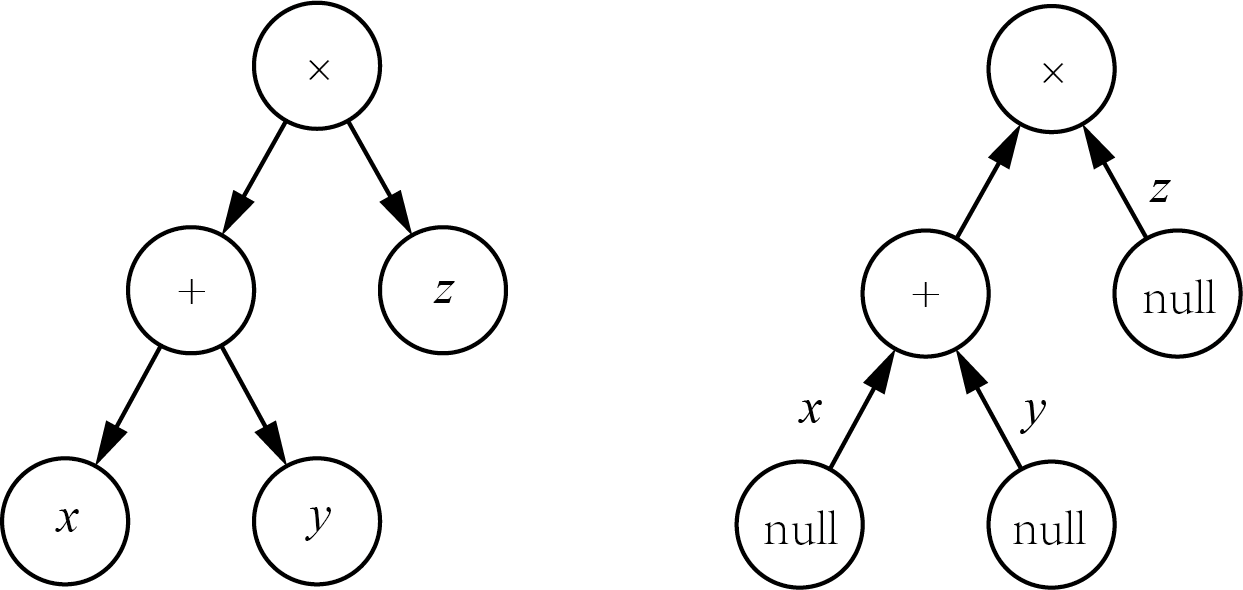
\includegraphics[width=0.5\textwidth]{assets/tree.png}
  \caption{$(x+y)*z$}
\end{figure}

上图中两个画法明显的不同在于对数值$x,y,z$的处理上,一个把它们放置在$\bigcirc$上,
一个放置在$\rightarrow$上。其实,两者并无明显不同。$\rightarrow$代表“取”或“送”
数据的数据流,这在两幅图中都有所体现。不同的是,左图认为\textbf{\textit{Scalar}}
也是一种运算\textbf{\textit{Operator}}。我们可以把这种对于Scalar的操作,看成是
$\exists$。所以,左图中左子树可以读作:$\exists x \& y, x+y$。

在计算图中,我们要适应以下画法:

\begin{figure}[h!]
  \centering
  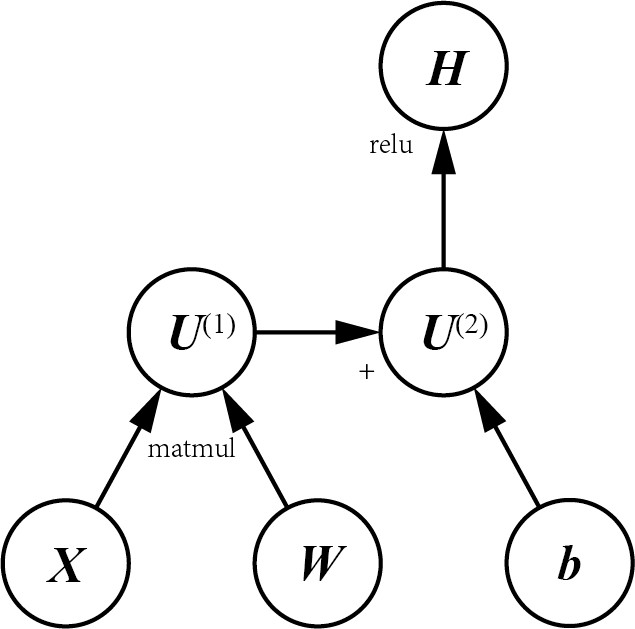
\includegraphics[width=0.25\textwidth]{assets/compute_graph.png}
  \caption{$\mathbf{H}=\max(0,\mathbf{XW}+\mathbf{b})$}
\end{figure}

又有一些不同,但其实并无差别。如果非要找一个可以讲讲的差别,那就是在计算图中临时变量
终于拥有了姓名,而不再是临时变量。在实际的编程中,临时变量的创建和销毁也需要占用大量
的系统资源。编写高性能运算的程序,不得不考虑临时变量的创建和销毁过程。关于这方面的一
个简单讨论,可以阅读\href{https://github.com/dmlc/mshadow/tree/master/guide/exp-template}
{Expression Template Tutorial - Mshadow Guide}。深度学习中的计算图站在一个比
较宏观的视角来看待各个算法,是一种各个算法的组织形式,而不是算法实现的数学细节。因此,
“神经网络领域里大量的研究和开发是\textbf{发明计算图的新结构},而并非发明崭新的算法”。

真实应用的计算图往往比第一个动图中的还要复杂,而且不同的计算$\bigcirc$可能分布于不同
的线程、不同的计算节点。因此,我们需要对各个$\bigcirc$进行调度,让他们依次准备好数据
,并推送给下游的$\bigcirc$。这时候,就是拓扑排序派上用场的时候了。它根据依赖关系,把
各个$\bigcirc$执行的优先级顺序进行确定,并依次执行。这样,\textbf{下游节点计算时需
要的数据,上游节点正好都准备好了}。无论在Forward还是Backward中,利用拓扑排序进行调度
的方法都十分有用。

\section{拓扑排序}
拓扑排序就像是月老同志,为大家连接好了姻缘线。你喜欢他/她的同时,他/她正好也喜欢你,岂
不美哉。所以,这是个好算法。
实现拓扑排序的方法主要有两种:\textbf{Kahn算法}和\textbf{深度优先搜索}。Kahn算法的
伪代码如下:

\begin{tcolorbox}
  L ← Empty list that will contain the sorted elements\\
  S ← Set of all nodes with no incoming edge\\
  -while S is non-empty do\\
  -\quad remove a node n from S\\
  -\quad add n to \textcolor{red}{\textbf{tail}} of L\\
  -\quad for each node m with an edge e from n to m do\\
  -\quad \quad remove edge e from the graph\\
  -\quad \quad if m has no other incoming edges then\\
  -\quad \quad \quad insert m into S\\
  -if graph has edges then\\
  -\quad return error   (graph has at least one cycle)\\
  -else\\
  -\quad return L   (a topologically sorted order)
\end{tcolorbox}

深度优先搜索的伪代码如下:
\begin{tcolorbox}
  L ← Empty list that will contain the sorted nodes\\
  -while exists nodes without a permanent mark do\\
  -\quad select an unmarked node n\\
  -\quad visit(n)
\end{tcolorbox}

\begin{tcolorbox}
  -function visit(node n)\\
  -\quad if n has a permanent mark then return\\
  -\quad if n has a temporary mark then stop   (not a DAG)\\
  -\quad mark n with a temporary mark\\
  -\quad for each node m with an edge from n to m do\\
  -\quad \quad visit(m)\\
  -\quad remove temporary mark from n\\
  -\quad mark n with a permanent mark\\
  -\quad add n to \textcolor{red}{\textbf{head}} of L
\end{tcolorbox}
这其中的一个坑,在上述伪代码中用\textcolor{red}{\textbf{红色加粗}}字体标记出来
了。其实,深度优先搜索对顶点的处理有三种顺序:1)前序;2)后序;3)逆后序。在拓扑排
序中的这种深度优先搜索属于3)逆后序。

\section{参考资料}
\begin{itemize}
  \item \href{https://www.tensorflow.org/guide/graphs}{Graphs and Sessions | Tensorflow}
  \item \href{https://wuyuans.com/2012/10/mathematical-symbols}{数学表示法}
  \item \href{https://en.wikipedia.org/wiki/Topological_sorting}{Topological sorting}
  \item \href{https://www.jianshu.com/p/b59db381561a}{什么是拓扑排序}
  \item \href{https://www.jianshu.com/p/ece68117538e}{3.控制流与实现思路}
\end{itemize}


\end{document}
